% v9 (2026-09-24): the head-to-head is now Table~\ref{tab:served}, by serving configuration and
% budget, every cell an order-averaged paired difference inside one judge pass on text with the
% prompt-tail echo removed (caution (bc)); Figure~\ref{fig:breadth} is selection against its OWN
% anchor only. v8 kept as output/review_audit/pre_main_2026-09-24/experiments.tex.
% Numbers: results/served_opponent.csv (Table 1), frontier_levels.csv, h2h_length_control.csv,
% selection_breadth_deecho.csv, selection_verifiable_*.csv, order_averaged_h2h_deecho.csv.

\section{Experiments}\label{sec:experiments}

\subsection{Setup}\label{sec:setup}

A certificate is worth nothing if the mechanism it certifies serves worse text, so we measure
selection against the metered decoder at the anchor its authors evaluate, \texttt{TinyComma-1.8B}
\citep{he2026anchored,kandpal2025commonpile}: trained only on openly licensed text, and sharing the
risky model's tokenizer, which the token-level meter needs. Their byte-level variant for mismatched vocabularies \citep{hayase2026bytesampler} we ran as released
at their recommended pair, Comma-7B with the $70$B base (Appendix~\ref{app:anchoredbyte}). \texttt{Llama-3.1-8B-Instruct} \citep{grattafiori2024llama3} is served
as the released logs of an earlier audit serve it --- a text continuer, without its chat template,
at temperature $1.0$ and no repetition penalty --- and \texttt{Llama-3.1-70B} base, the authors' own
pair, at the same temperature where they use $0.7$ and a penalty of $1.1$. The workload is $500$
ordinary prompts, none from the protected corpus: $200$ general-knowledge questions and $150$
WritingPrompts premises \citep{fan2018writingprompts} under a fixed \texttt{Complete the prefix:}
header, and $150$ FactScore biography requests \citep{min2023factscore}
(Table~\ref{tab:promptset}). Utility is a pairwise judgement against one fixed opponent, the
unconstrained risky model's own draw, shown in \emph{both} orders and averaged, so position is
removed by construction and $0.5$ is parity with the risky model. The
pre-specified judge~B is \texttt{Phi-3.5-mini-instruct} \citep{abdin2024phi3}; judge~A,
\texttt{Qwen2.5-7B-Instruct} \citep{qwen2025qwen25}, supplies the reward and never scores an arm it
selected; judge~C is the opponent's own checkpoint, a self-preference risk
\citep{panickssery2024llm}. Every band below was fixed before its run, and the first cost us
a claim.

\subsection{Main results}\label{sec:main-results}
\textbf{The scorer decides, and the obvious one fails.} The first scorer we specified in advance
was the risky model's own per-token log-likelihood --- the objective anchored decoding tilts toward
--- and it fails, moving judged utility by $-0.006$ at $n=8$ against a band fixed in advance of
$+0.077$. A circular oracle over the same eight draws reaches $+0.488$ (Appendix~\ref{app:currency}) and
a non-circular one, selecting by judge~A and scoring with judge~B, $+0.081$ $[+0.034, +0.130]$, so
what fails is the objective and not the budget; handed the same reward on TriviaQA the meter gains
nothing (Table~\ref{tab:parity}). The deployable scorer never consults the risky
model: a \emph{pointwise} reward, $\log p(\text{Yes}) - \log p(\text{No})$ from
\texttt{Qwen2.5-7B-Instruct} on one fixed template, under which judged utility is monotone in
$\log n$ (Figure~\ref{fig:selection}b) and judge~C agrees at $n=64$, $+0.117$ $[+0.070, +0.164]$.
The certificate is $4.159$ nats at $n=64$ under the pathwise
order and $\log 64 - 63/64 = 3.175$ under the sharper KL one \citep{beirami2025bestofn}; both are
\emph{bounds}, attained only for a tie-free score and unrepeated strings
(Appendix~\ref{app:realisedkl}), so every comparison below sets selection's bound against the
meter's \emph{measured} spend, the conservative direction.

\begin{table}[t]
\centering\footnotesize
\caption{\textbf{Selection against the metered decoder, by how the risky model is served.}
Order-averaged judge-B levels against one opponent per block, the risky model's own draw
($0.5$ = parity); $500$ prompts, temperature $1.0$, no repetition penalty. \emph{binds}: share of steps at which the budget is active; $K/S_w$: the
certificate against a $50$-token window ($S_w = 159.8$ nats), which says nothing at or above $1$.
Last column: selection at $n=64$ ($3.175$ nats, a bound) minus the meter, paired over prompts,
$95\%$ interval. Levels compare within a block only (Appendix~\ref{app:served}).}
\label{tab:served}
\setlength{\tabcolsep}{4.5pt}
\begin{tabular}{@{}lrrrrr@{}}
\toprule
risky model, as served & $k$ & binds & $K/S_w$ & meter & selection $-$ meter \\
\midrule
\multicolumn{6}{@{}l}{\emph{opponent: the $8$B-Instruct without its chat template; anchor alone $0.439$, selection $0.555$}} \\
$8$B-Instruct, continuing text & $0.5$ & $48.1\%$ & $0.63$ & $0.436$ & $+0.1195$ $[+0.0955, +0.1435]$ \\
 & $1$ & $5.5\%$ & $1.25$ & $0.456$ & $+0.0995$ $[+0.074, +0.1245]$ \\
 & $10$ & $0.008\%$ & $12.5$ & $0.490$ & $+0.0655$ $[+0.040, +0.092]$ \\
$70$B base (the authors' pair) & $0.5$ & $26.5\%$ & $0.63$ & $0.429$ & $+0.1265$ $[+0.103, +0.1495]$ \\
 & $1$ & $6.3\%$ & $1.25$ & $0.433$ & $+0.1225$ $[+0.098, +0.146]$ \\
 & $20$ & $0.00\%$ & $25.0$ & $0.451$ & $+0.1040$ $[+0.080, +0.1285]$ \\
\midrule
\multicolumn{6}{@{}l}{\emph{opponent: the $8$B-Instruct through its chat template; anchor alone $0.238$, selection $0.363$}} \\
$8$B-Instruct, chat template & $1$ & $15.7\%$ & $1.25$ & $0.322$ & $+0.0410$ $[+0.012, +0.0705]$ \\
 & $10$ & $0.16\%$ & $12.5$ & $0.501$ & $-0.1380$ $[-0.167, -0.107]$ \\
\bottomrule
\end{tabular}
\end{table}

\textbf{Against the metered decoder, the sign is set by how the risky model is served, and the
budget never pays for the difference} (Table~\ref{tab:served}). When the risky model continues
text, selection at $n=64$ is judged better than the meter at every budget we ran: by $+0.0655$
$[+0.040, +0.092]$ at $k=10$, where the meter serves the risky model's own distribution at
$99.99\%$ of steps and spends a measured $171.3$ nats, and by $+0.1195$ $[+0.0955, +0.1435]$ at
$k=0.5$, where its budget binds on half the steps and it is indistinguishable from its own anchor
($-0.0030$ $[-0.0235, +0.018]$). On the registered statistic, gains over each arm's own anchor-alone
control, selection gains $+0.1015$ $[+0.0765, +0.1260]$ for $3.175$ nats and the metered decoder
$+0.0510$ $[+0.025, +0.076]$ for $171.3$, a difference of $+0.0505$ $[+0.0155, +0.0860]$ at one fifty-fourth of the divergence, and
$+0.0495$ $[+0.0175, +0.0800]$ with every arm re-drawn on fresh seeds. The authors' $70$B pair repeats it at every budget, and at this
temperature the $70$B base is itself judged no better than the anchor, $+0.019$ $[-0.004, +0.042]$.
Served through its chat template the
$8$B is a stronger opponent --- it beats its own templateless text by $0.184$ --- and there the $k=10$ meter, which \emph{is} that model at
$99.84\%$ of steps, wins by $0.138$, while at $k=1$ it loses. \textbf{Every cell the meter wins is certified at $K/S_w \ge 1.25$
--- at nothing --- and wherever $K/S_w < 1$ the meter is judged indistinguishable from its own
anchor.}

\subsection{Ablations and robustness}\label{sec:ablations}

\looseness=-1 \textbf{The difference is not the judge, the length or the empty draws.} Single-order gains are
dominated by position --- the same two texts win $261$ of $500$ shown second and $24$ shown first ---
and a re-run at a different $n$-grid moves one by $0.04$ to $0.07$, so every head-to-head is
order-averaged. Re-scoring the same texts, five judges,
$3.8$--$72$B in four families, put the $k=10$ difference positive: it replicates under four judges
and is bounded below $0.03$ under the one clean frontier judge, \texttt{Mixtral-8x7B}
\citep{jiang2024mixtral}, whose interval straddles zero (Table~\ref{tab:h2hrepeat}). It replicates
across judges, not across opponents or workloads: a stronger fixed opponent dissolves it, unresolved
from strength $0.773$ up (Table~\ref{tab:opponentladder}), as does moving off prefix completion ---
on two public book corpora selection wins at a binding budget, on AlpacaEval the meter wins,
$-0.0329$ $[-0.0528, -0.0127]$ (Appendix~\ref{app:workload}). The meter writes
twice selection's words, and the difference survives length control \citep{dubois2024length},
$+0.0605$ $[+0.0236, +0.0971]$, and restriction to the $414$ prompts whose anchor controls are both
non-empty, $+0.0441$ $[+0.0024, +0.0864]$ (Appendix~\ref{app:served}; both post hoc).

\looseness=-1 \textbf{An adversarial scorer leaks nothing the anchor does not.} No selector can do better than
the pool's best draw, and over nine arms --- six anchors, a paraphrase event, an attacker scoring by
the \emph{memorising model's own likelihood}, and \texttt{Llama-3.1-70B} --- near-verbatim recall of
the best draw reads $0.0000$ at every $n$ to $64$ and at $n=256$, on every passage and at all six
anchors, against the memoriser alone at $0.3925$ mean and $0.8154$ maximum; the $70$B, which memorised
\emph{Harry Potter} in pre-training, recovers $0.2475$ unaided and reproduces two \emph{in full}. The zero verifies the anchor, not
the mechanism, and on $100$ passages bounds the per-passage rate below $3.0\%$ at $95\%$. Over twelve deliberately contaminated anchors the realised factor at
$n=64$ is $1.0$ to $7.0$, and $1.0$ to $3.0$ on a second draw, not the $64$ permitted
(Figure~\ref{fig:safety}, Table~\ref{tab:extraction}).

\begin{figure}[t]
\centering
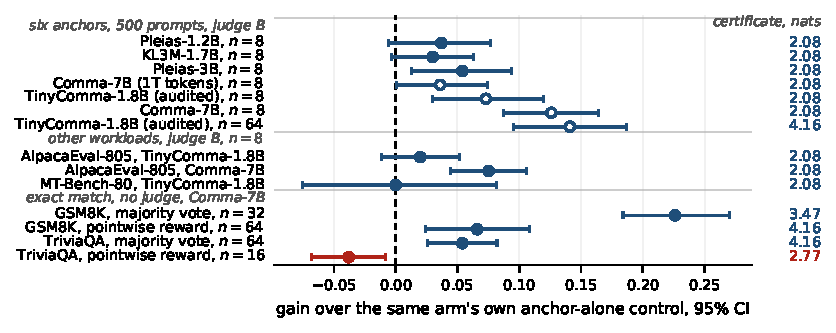
\includegraphics[width=0.78\textwidth]{figures/selection_breadth_forest.pdf}
\caption{\textbf{Selection against its own anchor.} Gain over \emph{that arm's own} anchor-alone
draw, single-order, $95\%$ interval, judged on the repaired text; right, the \emph{entire} budget in nats.
Open markers miss the admission criterion, over $5\%$ empty completions on the true generations
(TinyComma $14.6\%$ and $12.8\%$, Comma-7B $18.4\%$, Comma-1T $31.6\%$); on non-empty prompts their
gains move by at most $0.012$. MT-Bench's $80$ items resolve nothing at a half-width of $0.08$, and the
pointwise reward turns over with $n$ (Figure~\ref{fig:judgefree}).}
\label{fig:breadth}
\end{figure}

\textbf{Six anchors, two more workloads, and tasks with no judge at all.}
Figure~\ref{fig:breadth} is selection against its own anchor. A safe model must be trained without
the protected work, which rules out the open-\emph{data} families and leaves the openly
\emph{licensed} ones \citep{kandpal2025commonpile,langlais2026commoncorpus,bommarito2025kl3m}, the
largest being Comma-7B: the ceiling is the licensing frontier, not our compute, and the check of
Appendix~\ref{app:vetting} reads $0.000$ at all six licensed anchors and above zero at both OLMo-2
models \citep{olmo2024olmo2}. At $n=8$ the gain excludes zero at four of six anchors in two
families (KL3M-1.7B's only on the recorded text, Comma-1T's only on the repaired), largest at Comma-7B, $+0.126$ $[+0.087, +0.164]$, and does not track the anchor's own level
($\rho = +0.543$ on the two-judge mean). \textbf{Two tasks need no judge}: on GSM8K
\citep{cobbe2021gsm8k} majority vote takes exact match from $0.320$ to $0.546$ for $3.47$ certified
nats, $3.4\times$ the pointwise reward's best lift, while on TriviaQA \citep{joshi2017triviaqa} that
reward \emph{falls} with $n$ (Figure~\ref{fig:judgefree}, Appendix~\ref{app:judgefree}), and on MMLU
\citep{hendrycks2021mmlu}, a forced choice, both lift. What saturates is the scorer, not the
mechanism, which is why the headline rule is the one with nothing to overoptimise against. The
ceiling binds across anchors, not within one: across domains inside one anchor the same test is
inseparable from a no-effect null (Appendix~\ref{app:limitations}).
